%%%%%%%%%%%%%%%%%%%%%%%%%%%%%%%%%%%%%%%%%%%%%%%%%%%%%%
% A Beamer template for Ritsumeikan University       %
% Author: Ming-Hao Xu (Xu Minghao)                   %
% Date:   April 2022.                                %
% LPPL Licensed.                                     %
%%%%%%%%%%%%%%%%%%%%%%%%%%%%%%%%%%%%%%%%%%%%%%%%%%%%%%

\documentclass{beamer}
\usepackage{hyperref}

\usepackage[UTF8]{ctex}
\usepackage[T1]{fontenc}

% other packages
\usepackage{latexsym,amsmath,xcolor,multicol,booktabs,calligra}
\usepackage{graphicx,pstricks,listings,stackengine}
\usefonttheme[onlymath]{serif}

% dummy text; remove it when working on this template
\usepackage{lipsum}

\author{Ebola}
\title{OI中的数值分析}
\institute{
    Institute of Mathematics, \\
    Zhejiang University.
}
\date{July, 2023}
\usepackage{Ritsumeikan}

% defs
\def\cmd#1{\texttt{\color{red}\footnotesize $\backslash$#1}}
\def\env#1{\texttt{\color{blue}\footnotesize #1}}
\definecolor{deepblue}{rgb}{0,0,0.5}
\definecolor{deepred}{rgb}{0.6,0,0}
\definecolor{deepgreen}{rgb}{0,0.5,0}
\definecolor{halfgray}{gray}{0.55}

\lstset{
    basicstyle=\ttfamily\tiny,
    keywordstyle=\bfseries\color{deepblue},
    emphstyle=\ttfamily\color{deepred},    % Custom highlighting style
    stringstyle=\color{deepgreen},
    numbers=left,
    numberstyle=\small\color{halfgray},
    rulesepcolor=\color{red!20!green!20!blue!20},
    frame=shadowbox,
}


\begin{document}

\begin{frame}
    \titlepage
\end{frame}

\begin{frame}
    \tableofcontents[sectionstyle=show,subsectionstyle=show/shaded/hide,subsubsectionstyle=show/shaded/hide]
\end{frame}

\section{牛顿迭代}

\begin{frame}{问题引入}
    给定一个连续可微的函数$f(x)$,例如
    \begin{equation*}
        f(x)=x^5-2x^4+3x^3-4x^2+5x-6
    \end{equation*}
    如何求方程$f(x)=0$的解?

    提示:$f(0)=-6,\;f(2)=12$
\end{frame}

\begin{frame}{牛顿迭代法}
    \begin{figure}[H]
        \centering
        \begin{minipage}[t]{0.48\textwidth}
            \centering
            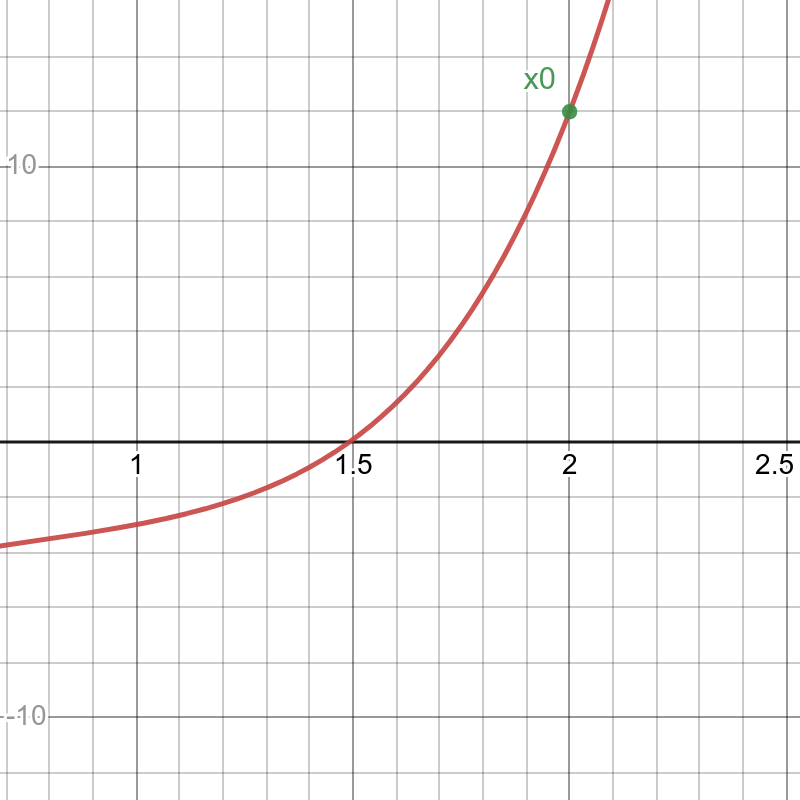
\includegraphics[width=0.9\textwidth]{pic/newton1.png}
        \end{minipage}
        \begin{minipage}[t]{0.48\textwidth}
            \centering
            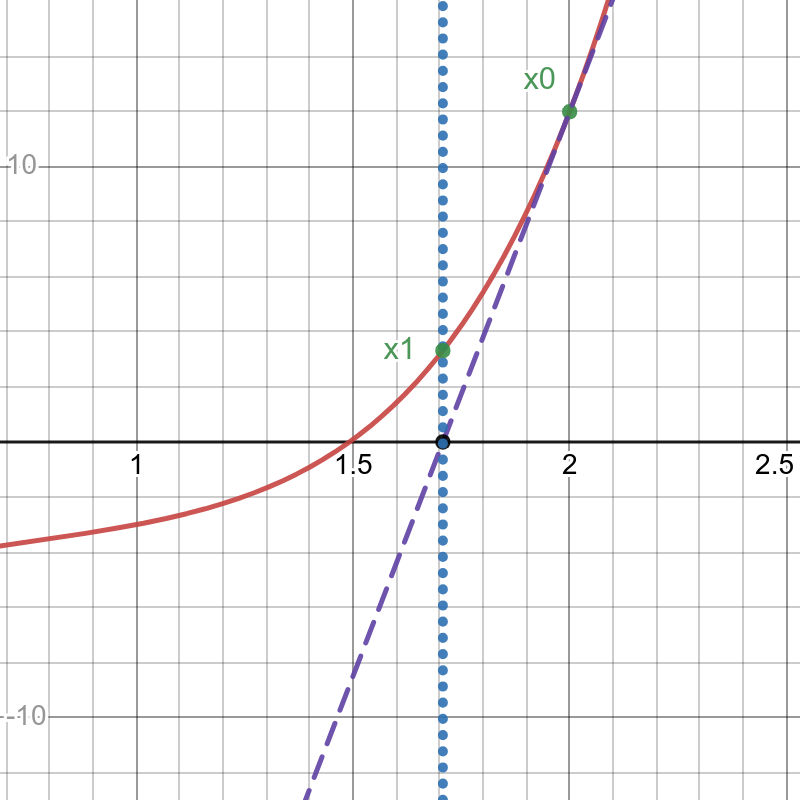
\includegraphics[width=0.9\textwidth]{pic/newton2.png}
        \end{minipage}
    \end{figure}
    \begin{align*}
        x_0 &= 2\\
        x_1 &= x_0 - \frac{f(x_0)}{f'(x_0)} = 1.7073
    \end{align*}
\end{frame}

\begin{frame}{牛顿迭代法}
    \begin{figure}[H]
        \centering
        \begin{minipage}[t]{0.48\textwidth}
            \centering
            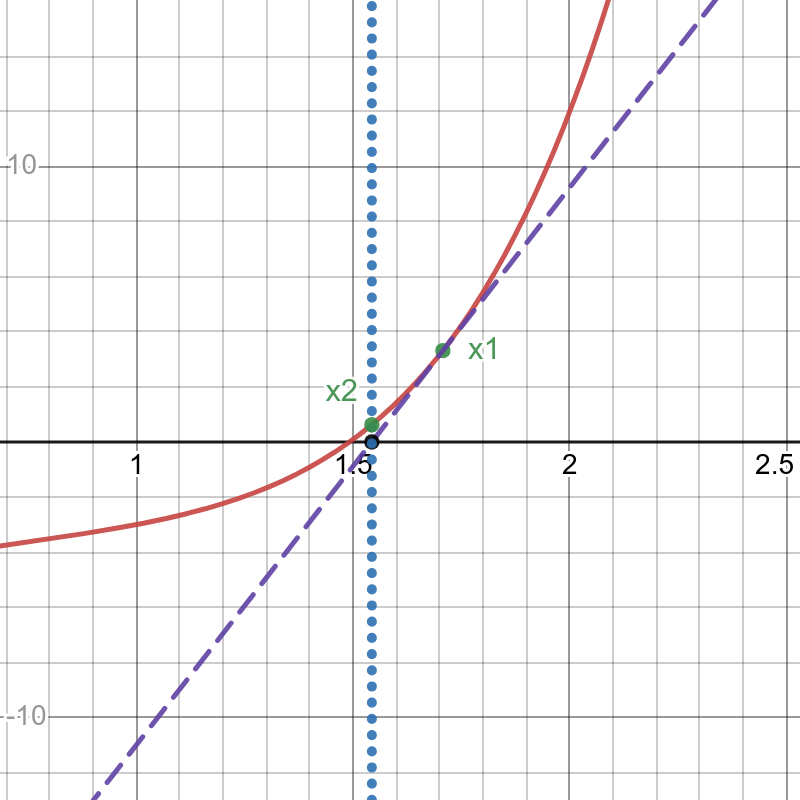
\includegraphics[width=0.9\textwidth]{pic/newton3.png}
        \end{minipage}
        \begin{minipage}[t]{0.48\textwidth}
            \centering
            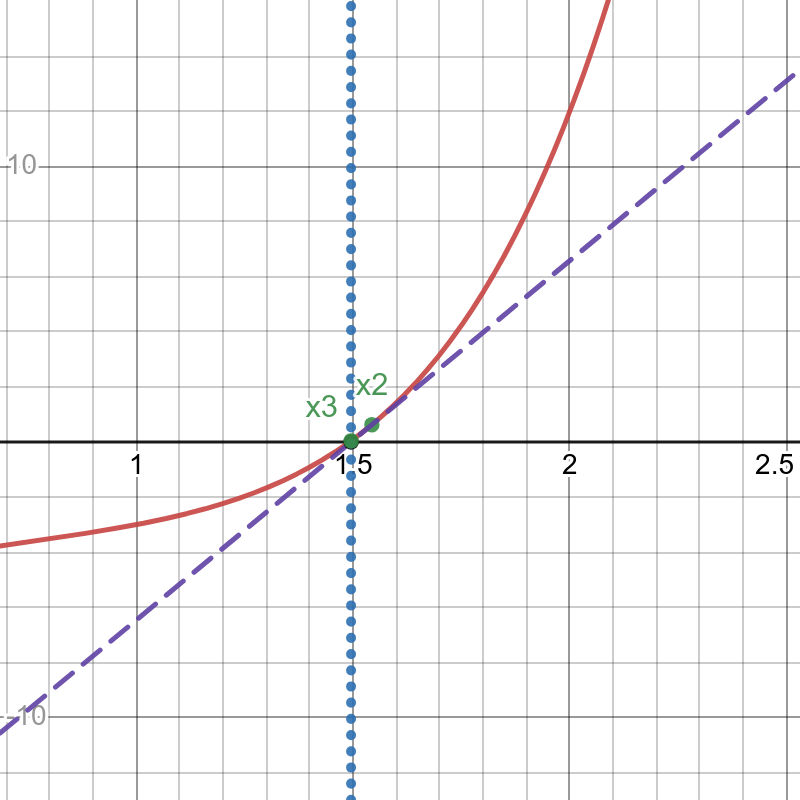
\includegraphics[width=0.9\textwidth]{pic/newton4.png}
        \end{minipage}
    \end{figure}
    \begin{align*}
        x_2 &= x_1 - \frac{f(x_1)}{f'(x_1)} = 1.5433\\
        x_3 &= x_2 - \frac{f(x_2)}{f'(x_2)} = 1.4953
    \end{align*}
\end{frame}

\begin{frame}{效率比较}
    $f(x)=x^5-2x^4+3x^3-4x^2+5x-6$的零点为$x^*=1.491797988139901$,用不同的方法求解。

    \begin{figure}[H]
        \centering
        \begin{minipage}[t]{0.48\textwidth}
            \centering
            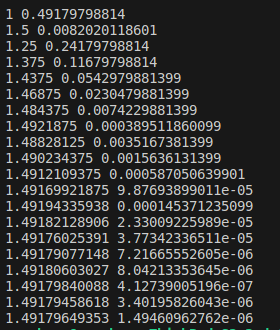
\includegraphics[width=0.9\textwidth]{pic/bisection.png}
            \caption{二分法}
        \end{minipage}
        \begin{minipage}[t]{0.48\textwidth}
            \centering
            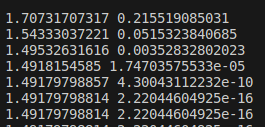
\includegraphics[width=0.9\textwidth]{pic/newton.png}
            \caption{牛顿迭代法}
        \end{minipage}
    \end{figure}
\end{frame}

\section{高斯消元}

\begin{frame}{线性方程组}
    我们现在有一个线性方程组
    \begin{equation*}
        \left\{
            \begin{array}{l}
                a_{11}x_1+a_{12}x_2+\cdots +a_{1n}x_n = b_1\\
                a_{21}x_1+a_{22}x_2+\cdots +a_{2n}x_n = b_2\\
                \vdots\\
                a_{n1}x_1+a_{n2}x_2+\cdots +a_{nn}x_n = b_n
            \end{array}
        \right.
    \end{equation*}

    我们可以用二维数组来存这个方程组:
    \begin{equation*}
        A=\begin{bmatrix}
            a_{11} & a_{12} & \cdots & a_{1n} & b_1\\
            a_{21} & a_{22} & \cdots & a_{2n} & b_2\\
            \vdots & \vdots & \ddots & \vdots & b_3\\
            a_{n1} & a_{n2} & \cdots & a_{nn} & b_4
        \end{bmatrix}
    \end{equation*}
\end{frame}

\begin{frame}{例子}
    \begin{equation*}
        \left\{
            \begin{array}{l}
                3x_1 + 2x_2 + x_3 = 1\\
                2x_1 - 3x_2 + 2x_3 = 2\\
                x_1 + x_2 - x_3 = 2
            \end{array}
        \right. \qquad 
        A=\begin{bmatrix}
            3 & 2 & 1 & 1\\
            2 & -3 & 2 & 2\\
            1 & 1 & -1 & 2
        \end{bmatrix}
    \end{equation*}

    第一行乘$\frac{1}{3}$:
    \begin{equation*}
        \left\{
            \begin{array}{l}
                x_1 + \frac{2}{3}x_2 + \frac{1}{3}x_3 = \frac{1}{3}\\
                2x_1 - 3x_2 + 2x_3 = 2\\
                x_1 + x_2 - x_3 = 2
            \end{array}
        \right. \qquad 
        A=\begin{bmatrix}
            1 & \frac{2}{3} & \frac{1}{3} & \frac{1}{3}\\
            2 & -3 & 2 & 2\\
            1 & 1 & -1 & 2
        \end{bmatrix}
    \end{equation*}

    第二行减两倍的第一行、第三行减第一行:
    \begin{equation*}
        \left\{
            \begin{array}{l}
                x_1 + \frac{2}{3}x_2 + \frac{1}{3}x_3 = \frac{1}{3}\\
                - \frac{13}{3}x_2 + \frac{4}{3}x_3 = \frac{4}{3}\\
                \frac{1}{3}x_2 - \frac{4}{3}x_3 = \frac{5}{3}
            \end{array}
        \right. \qquad 
        A=\begin{bmatrix}
            1 & \frac{2}{3} & \frac{1}{3} & \frac{1}{3}\\
            0 & -\frac{13}{3} & \frac{4}{3} & \frac{4}{3}\\
            0 & \frac{1}{3} & -\frac{4}{3} & \frac{5}{3}
        \end{bmatrix}
    \end{equation*}
\end{frame}

\begin{frame}{例子}
    第二行乘$-\frac{3}{13}$:
    \begin{equation*}
        \left\{
            \begin{array}{l}
                x_1 + \frac{2}{3}x_2 + \frac{1}{3}x_3 = \frac{1}{3}\\
                x_2 - \frac{4}{13}x_3 = -\frac{4}{13}\\
                \frac{1}{3}x_2 - \frac{4}{3}x_3 = \frac{5}{3}
            \end{array}
        \right. \qquad 
        A=\begin{bmatrix}
            1 & \frac{2}{3} & \frac{1}{3} & \frac{1}{3}\\
            0 & 1 & -\frac{4}{13} & -\frac{4}{13}\\
            0 & \frac{1}{3} & -\frac{4}{3} & \frac{5}{3}
        \end{bmatrix}
    \end{equation*}

    第三行减$\frac{1}{3}$倍的第二行:
    \begin{equation*}
        \left\{
            \begin{array}{l}
                x_1 + \frac{2}{3}x_2 + \frac{1}{3}x_3 = \frac{1}{3}\\
                x_2 - \frac{4}{13}x_3 = -\frac{4}{13}\\
                - \frac{16}{13}x_3 = \frac{23}{13}
            \end{array}
        \right. \qquad 
        A=\begin{bmatrix}
            1 & \frac{2}{3} & \frac{1}{3} & \frac{1}{3}\\
            0 & 1 & -\frac{4}{13} & -\frac{4}{13}\\
            0 & 0 & -\frac{16}{13} & \frac{23}{13}
        \end{bmatrix}
    \end{equation*}

    第三行乘$-\frac{13}{16}$:
    \begin{equation*}
        \left\{
            \begin{array}{l}
                x_1 + \frac{2}{3}x_2 + \frac{1}{3}x_3 = \frac{1}{3}\\
                x_2 - \frac{4}{13}x_3 = -\frac{4}{13}\\
                x_3 = -\frac{23}{16}
            \end{array}
        \right. \qquad 
        A=\begin{bmatrix}
            1 & \frac{2}{3} & \frac{1}{3} & \frac{1}{3}\\
            0 & 1 & -\frac{4}{13} & -\frac{4}{13}\\
            0 & 0 & 1 & -\frac{23}{16}
        \end{bmatrix}
    \end{equation*}
\end{frame}

\begin{frame}[fragile]{代码}
    \begin{minipage}{\linewidth}
    \begin{lstlisting}[language=c++]
    for(int i=1;i<=n;i++)
    {
        int pos=i;
        while(G[pos][i]==0&&pos<n) pos++;
        if(fabs(G[pos][i])<1e-12) return false;
        if(pos!=i)
            for(int j=1;j<=n+1;j++) swap(G[i][j],G[pos][j]);
        for(int j=i+1;j<=n;j++)
        {
            double t=G[j][i]/G[i][i];
            if(fabs(G[j][i])<1e-12) continue;
            for(int k=i;k<=n+1;k++)
                G[j][k]-=G[i][k]*t;
        }
    }
    for(int i=n;i>=1;i--)
    {
        for(int j=i+1;j<=n;j++)
            G[i][n+1]-=G[i][j]*ans[j];
        ans[i]=G[i][n+1]/G[i][i];
    }
    for(int i=1;i<=n;i++) printf("%.2lf\n",ans[i]);
    \end{lstlisting}
    \end{minipage}
\end{frame}

\begin{frame}{例题选讲:[CF24D] Broken Robot}
    \small 
    $n$ 行 $m$ 列的矩阵,现在在 $(x,y)$,每次等概率向左,右,下走或原地不动,但不能走出去,问走到最后一行期望的步数。

    注意,$(1,1)$ 是木板的左上角,$(n,m)$ 是木板的右下角。

    $1\le n,m\le 10^3$,$1\le x\le n$,$1\le y\le m$。

    \vspace{1em}\pause
    【题解】 设$f_{i,j}$表示从$(i,j)$出发,走到最后一行的期望步数

    \vspace{.5em}
    \pause
    设$j\neq 1$且$j\neq m$,那么
    \begin{equation*}
        f_{i,j}=\frac{1}{4}f_{i,j}+\frac{1}{4}f_{i,j-1}+\frac{1}{4}f_{i,j+1}+\frac{1}{4}f_{i+1,j}+1
    \end{equation*}

    此外
    \begin{align*}
        f_{i,1}&=\frac{1}{3}f_{i,1}+\frac{1}{3}f_{i,2}+\frac{1}{3}f_{i+1,1}+1\\
        f_{i,m}&=\frac{1}{3}f_{i,m}+\frac{1}{3}f_{i,m-1}+\frac{1}{3}f_{i+1,m}+1
    \end{align*}

    \vspace{.5em}
    \pause
    可以从下往上倒推,每一行的DP式子都是一个$m$元方程组,高斯消元求解即可。
\end{frame}

\begin{frame}{例题选讲:[HNOI2013] 游走}

给定一个 $n$ 个点 $m$ 条边的无向连通图,顶点从 $1$ 编号到 $n$,边从 $1$ 编号到 $m$。 

小 Z 在该图上进行随机游走,初始时小 Z 在 $1$ 号顶点,每一步小 Z 以相等的概率随机选择当前顶点的某条边,沿着这条边走到下一个顶点,获得等于这条边的编号的分数。当小 Z 到达 $n$ 号顶点时游走结束,总分为所有获得的分数之和。 现在,请你对这 $m$ 条边进行编号,使得小 Z 获得的总分的期望值最小。

\end{frame}

\begin{frame}{例题选讲:[HNOI2013] 游走}
    【题解】 记$d_i$表示点$i$的度数,若点$i$经过次数的期望是$f_i$,那么对于一条连接$(i,j)$的边$e$,经过$e$的次数期望为:
    \begin{equation*}
        g_e=\frac{g_i}{d_i}+\frac{g_j}{d_j}
    \end{equation*}

    现在来计算$f_i$
    \pause
    ,不难列出转移:
    \begin{equation*}
        f_i=\sum_{\text{边}(i,j),j\neq n} \frac{f_j}{d_j},\qquad i\neq 1
    \end{equation*}
    \begin{equation*}
        f_1=1+\sum_{\text{边}(1,j),j\neq n} \frac{f_j}{d_j}
    \end{equation*}

    这是一个线性方程组,高斯消元求解即可,复杂度$O(n^3)$.
\end{frame}

\begin{frame}{例题选讲:[HDU4870] Rating}
    \small 
    有两个账号,每次选取一个分数最低的账号进行游戏(如果两个账号分数一样,就用第一个帐号),有$p$的概率得1分,$1-p$的概率倒扣2分,最低0分,求有1个号到达20所需的游戏次数的期望。

    \vspace{1em}\pause
    【题解】 设$E_{i,j}$表示当前第一个帐号得分为$i$,第二个帐号得分为$j$,距离游戏结束期望还要多少步。

    \pause
    如果$i\leq j$:
    \begin{equation*}
        E_{i,j}=pE_{i+1,j}+(1-p)E_{\min(i-2,0),j}+1
    \end{equation*}

    如果$i>j$:
    \begin{equation*}
        E_{i,j}=pE_{i,j+1}+(1-p)E_{i,\min(j-2,0)}+1
    \end{equation*}

    \pause
    列出方程,高斯消元求解即可。
\end{frame}

\section{辛普森积分}

\begin{frame}{问题引入}
    给定一个函数$f(x)$和区间$[a,b]$,求
    \begin{equation*}
        \int_a^b f(x)\text{d}x
    \end{equation*}
    的近似值。
\end{frame}

\begin{frame}
    我们给出一个公式:
    \begin{equation*}
        I(a,b)=\frac{b-a}{6}\left(f(a)+4f\left(\frac{a+b}{2}\right)+f(b)\right)
    \end{equation*}
    
    假设$f(x)$是一个二次函数,那么恰好满足:
    \begin{equation*}
        \int_a^b f(x)\text{d}x=I(a,b)
    \end{equation*}

    如果$f(x)$不是二次函数呢?\pause
    我们可以计算$I(a,b),\;I\left(a,\frac{a+b}{2}\right),\;I\left(\frac{a+b}{2},b\right)$,如果
    \begin{equation*}
        \left|I(a,b)-\left(I\left(a,\frac{a+b}{2}\right)+I\left(\frac{a+b}{2},b\right)\right)\right| < \varepsilon
    \end{equation*}

    我们就认为我们的计算已经足够精确,将$I(a,b)$作为结果返回即可。否则,递归处理两个子区间。
\end{frame}

\begin{frame}[fragile]{代码}
    \begin{minipage}{\linewidth}
    \begin{lstlisting}[language=c++]
    double I(double l,double r)
    {
        double mid=(l+r)/2;
        return (F(l)+4*F(mid)+F(r))*(r-l)/6;
    }
    double simpson(double l,double r,double A)
    {
        double mid=(l+r)/2;
        double L=I(l,mid),R=I(mid,r);
        if(fabs(L+R-A)<eps) return L+R;
        return simpson(l,mid,L)+simpson(mid,r,R);
    }
    double simpson(double l,double r){return simpson(l,r,I(l,r));}
    \end{lstlisting}
    \end{minipage}
\end{frame}

\begin{frame}{例题选讲:圆的面积并}
    给定$n$,还有$n$个圆$(O_1,R_1),...,(O_n,R_n)$,求圆覆盖部分的面积之和。

    \pause
    【题解】 辛普森积分,转化为求直线$x=x_0$与所有圆的相交部分长度,$O(n)$求即可。
\end{frame}

\begin{frame}{例题选讲:洛谷P4526}
    给定$a$,求
    \begin{equation*}
        \int_0^\infty x^{\frac{a}{x}-x} \text{d}x
    \end{equation*}

    \pause
    \begin{figure}
        \begin{minipage}[t]{0.32\textwidth}
            \centering
            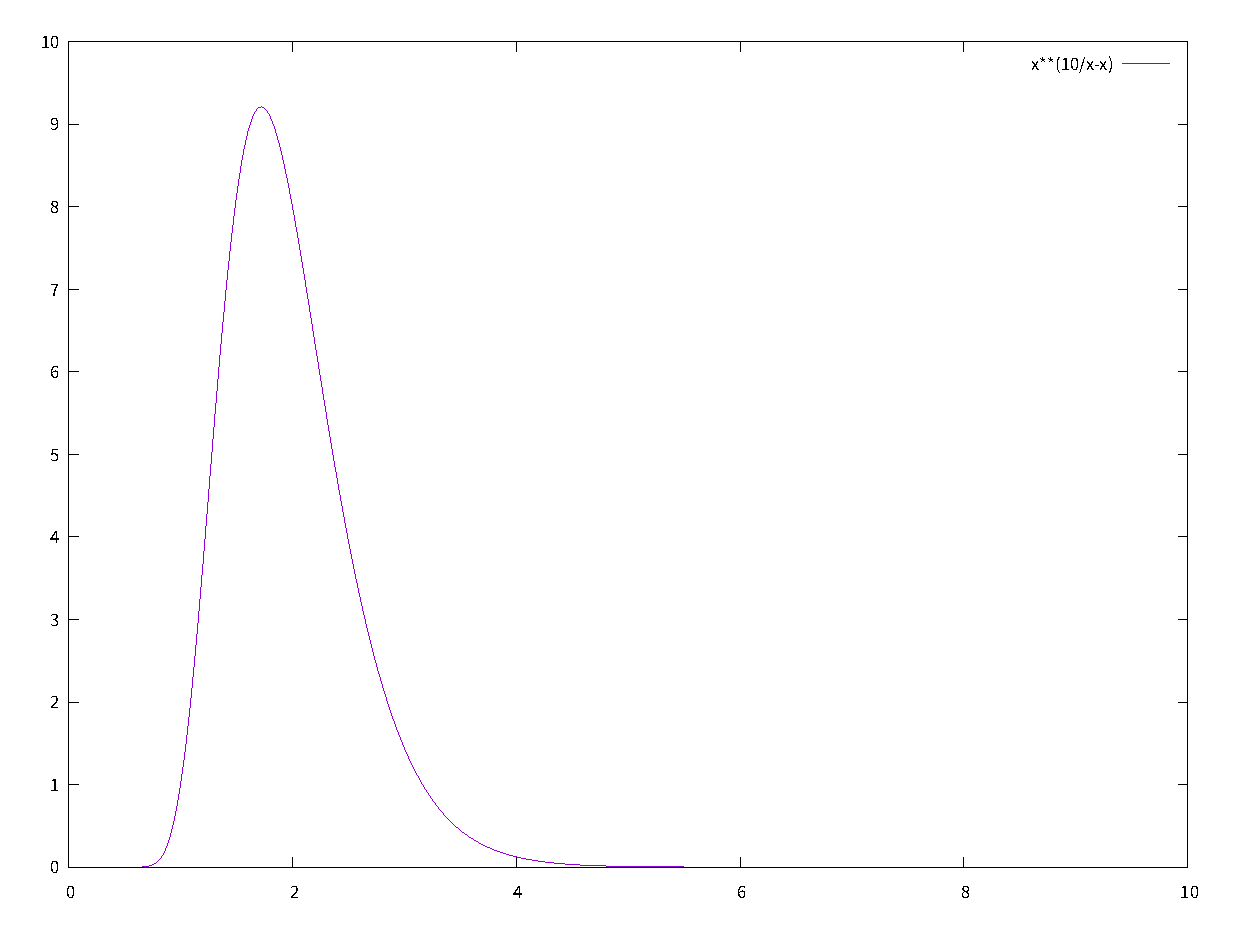
\includegraphics[width=0.95\textwidth]{pic/p4526-2.eps}
            \caption{$a=1$}
        \end{minipage}
        \begin{minipage}[t]{0.32\textwidth}
            \centering
            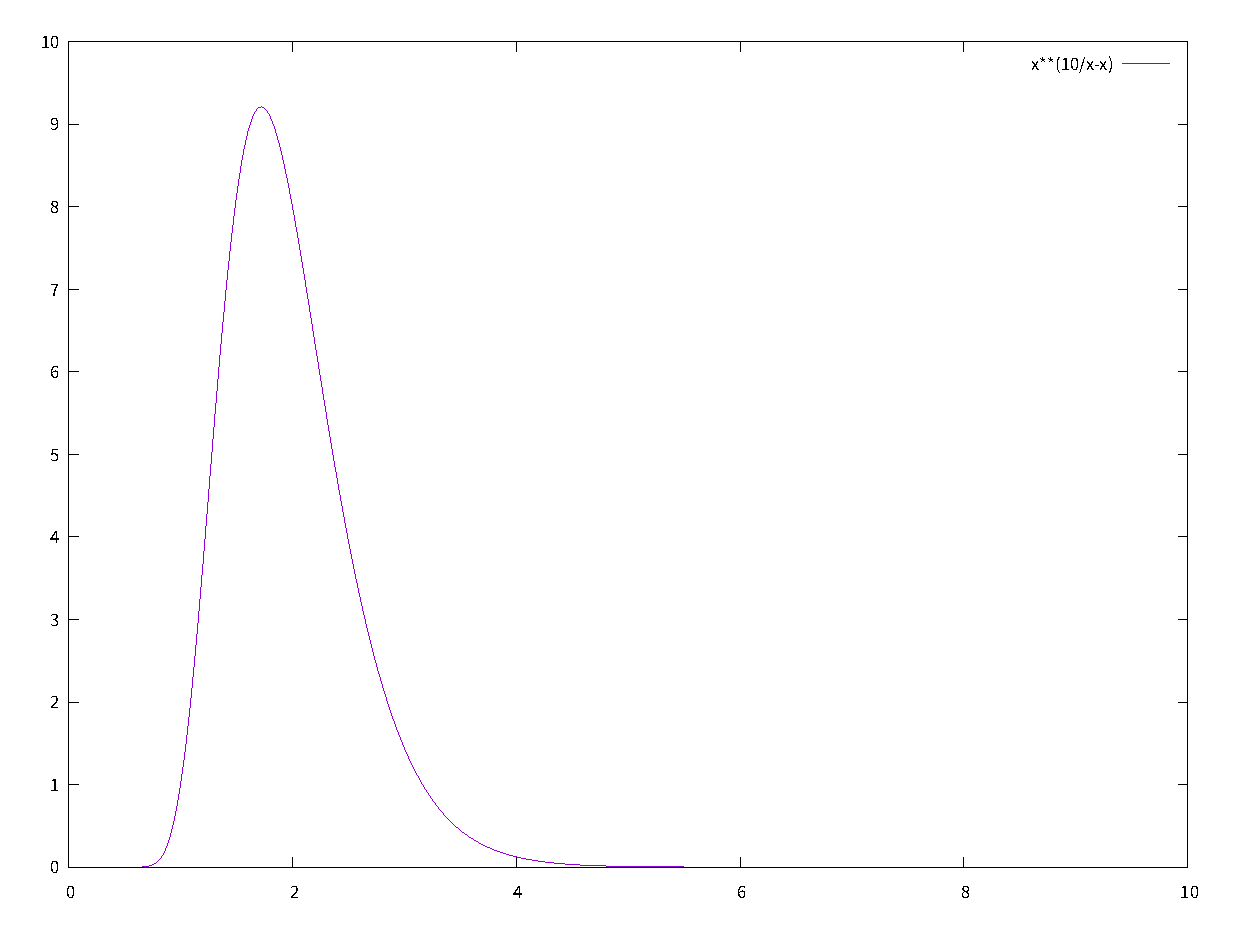
\includegraphics[width=0.95\textwidth]{pic/p4526-2.eps}
            \caption{$a=10$}
        \end{minipage}
        \begin{minipage}[t]{0.32\textwidth}
            \centering
            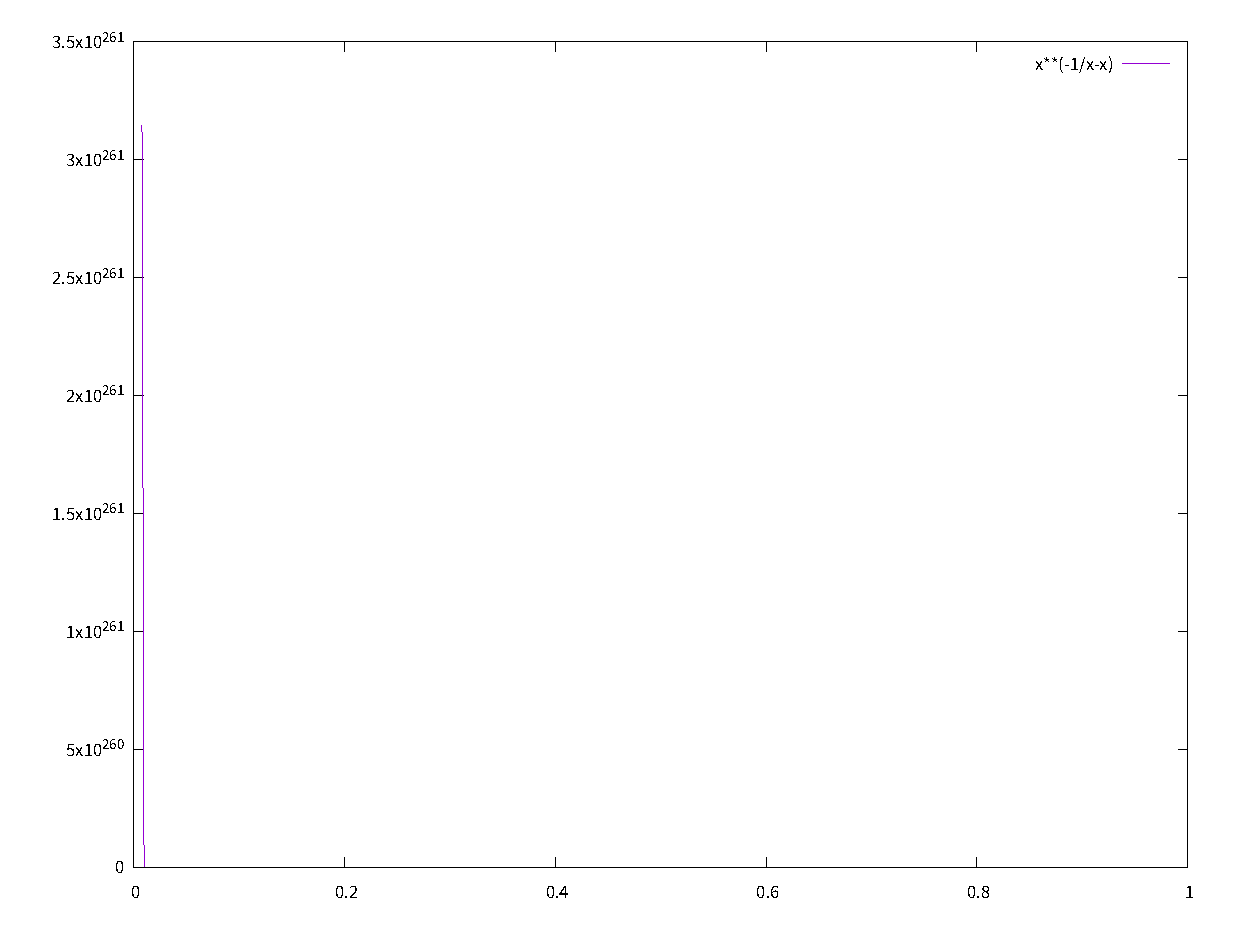
\includegraphics[width=0.95\textwidth]{pic/p4526-3.eps}
            \caption{$a=-1$}
        \end{minipage}
    \end{figure}

    \pause
    【题解】 $x>10$时函数值几乎为$0$,在$[\varepsilon,20]$区间上做辛普森积分即可。注意:$a<0$时积分发散。
\end{frame}

\begin{frame}{例题选讲:最短路期望}
    设$t$是一个在$[0,1]$中均匀分布的随机变量。给定一个有向图,$n$个点$m$条边,每条边的边长是$a_i+td_i$,求$1$到$n$的最短路径期望长度。

    $n\leq 1000,\; m\leq 2000$

    \pause
    \vspace{1em}
    【题解】 假如$t$是已知数,可以直接求最短路,记最短路长为$E(t)$。

    \pause
    \vspace{1em}
    用辛普森自适应积分计算
    \begin{equation*}
        \int_0^1 E(t) \text{d} t
    \end{equation*}
    
    即可
\end{frame}

\section{拉格朗日插值}

\begin{frame}{问题引入}
    给定一些点$(x_0,y_0),(x_1,y_1),...,(x_n,y_n)$,其中$x_0,x_1,...,x_n$两两不同,能否找到一个$n$次多项式$f(x)$,使$f(x_0)=y_0,f(x_1)=y_1,...,f(x_n)=y_n$?

    \vspace{1em}
    注意:我们并不需要计算$f(x)$的各项系数,只需求出$f(x^*)$的值,其中$x^*$是给定的。

    \vspace{1em}
    \pause 高斯消元:复杂度$O(n^3)$
\end{frame}

\begin{frame}{拉格朗日插值公式}
    对于给定的$(x_0,y_0),(x_1,y_1),...,(x_n,y_n)$,我们给出插值公式:
    \begin{equation*}
        f(x)=\sum_{i=0}^n y_i \prod_{j=1,\;j\neq i}^n \frac{x-x_j}{x_i-x_j}
    \end{equation*}

    不难验证$f(x_k)=y_k$,且$f(x)$是$n$次多项式。

    \pause
    求一个点值的复杂度:$O(n^2)$
\end{frame}

\begin{frame}{针对连续整数的特殊优化}
    假设给定的点是$(0,y_0),(1,y_1),...,(n,y_n)$,我们有:
    \begin{align*}
        f(x)&= \sum_{i=0}^n y_i \prod_{j=1,\;j\neq i}^n \frac{x-j}{i-j}\\
        &= \sum_{i=0}^n y_i \frac{(-1)^{n-i}A}{i!(n-i)!(x-j)}
    \end{align*}

    其中$A=\prod_{j=0}^n(x-j)$,可以$O(n)$预处理。总复杂度:$O(n)$
\end{frame}

\begin{frame}{例题选讲:自然数幂求和}
    求$1^k+2^k+...+n^k \mod 998244353$

    $k\leq 10^6,\;n\leq 10^9$

    \pause
    \vspace{1em}
    【题解】 设$f(m)=1^k+2^k+...+m^k$,$f(m)$是一个$k+1$次多项式。

    \pause
    \vspace{1em}
    求出$f(0),f(1),...,f(k+1)$,然后用拉格朗日插值求$f(n)$即可。复杂度$O(k\log k)$,其中$\log$来自快速幂。

\end{frame}

\begin{frame}{例题选讲:CF995F}
    给定一个$n$个点的树,以$1$为根,你要给每个节点分配权值$[1,d]$,使得子节点不超过父亲节点的权值,问有多少种分配方案。

    $n\leq 3000,\; d\leq 10^{9}$

    \pause
    \vspace{1em}
    【题解】 设$f_{u}(i)$表示$u$子树内权值大于等于$i$的方案数
    \pause
    \begin{equation*}
        f_{u}(i)=f_{u}(i+1)+\prod_{u\text{的子结点}v} f_{v}(i)
    \end{equation*}

    $d$太大了,怎么办?

    \pause
    \vspace{1em}
    $f_1(i)$是关于$i$的$n$次多项式。求出$f_1(1),f_1(2),...,f_1(n+1)$,然后用拉格朗日插值求$f_1(d)$即可。
\end{frame}

\begin{frame}{[集训队互测 2012] calc}
    \small 
    一个序列$a_1,a_2,...,a_n$是合法的,当且仅当:
    \begin{itemize}
        \item $a_1,a_2,...,a_n$都是$[1,k]$中的整数
        \item $a_1,a_2,...,a_n$互不相等
    \end{itemize}

    一个序列的值定义为它里面所有数的乘积,即$a_1\times a_2\times \cdots \times a_n$

    求不同合法序列的值的和对$p$取模后的结果。两个序列不同当且仅当它们任意一位不同。

    $n\leq 500,\;k\leq 10^9$

    \pause
    \vspace{1em}
    【题解】 首先可以假设$a_1<a_2<\cdots < a_n$,答案最后乘上$n!$即可

    \pause
    设$f_{i,j}$表示考虑完前$i$个数,且$a_i\leq j$时的答案
    \pause
    \begin{equation*}
        f_{i,j}=jf_{i-1,j-1} + f_{i,j-1}
    \end{equation*}

    最终答案是$n!f_{n,k}$,$k$太大了怎么办?

    \pause
    考虑令$f_{n,k}=f_n(k)$,可以验证$f_n(k)$是关于$k$的$2n$次多项式。求出前$2n+1$个值,拉格朗日插值即可。
\end{frame}

\section{快速傅里叶变换}

\begin{frame}
    给定多项式
    \begin{align*}
        f(x) &= a_0 + a_1x + a_2x^2 + \cdots + a_nx^n\\
        g(x) &= b_0 + b_1x + b_2x^2 + \cdots + b_mx^m
    \end{align*}
    求$h(x)=f(x)g(x)$的各项系数,记
    \begin{equation*}
        h(x) = c_0 + c_1x + c_2x^2 + \cdots  + c_{n+m}x^{n+m}
    \end{equation*}
    最简单的做法?
    \pause

    \begin{equation*}
        c_k=a_0b_k + a_1b_{k-1} + \cdots  + a_{k-1}b_1 + a_kb_0.
    \end{equation*}
    算一个$c_k$的复杂度是$O(k)$,算出所有$c_0,...,c_{n+m}$的复杂度为$O(n^2)$.
\end{frame}

\begin{frame}{傅里叶的思路}
    在拉格朗日插值中,我们知道了$n+1$个点可以唯一确定一个$n$阶多项式,加入我们取$N$个点,这里$N>n+m$,那么第一步(多点求值):我们计算
    \begin{align*}
        & f(x_1), f(x_2), ..., f(x_N)\\
        & g(x_1), g(x_2), ..., g(x_N)
    \end{align*}

    第二步(各点乘积):我们计算出
    \begin{align*}
        h(x_1)=f(x_1)g(x_1),\;h(x_2)=f(x_2)g(x_2),...,\;h(x_N)=f(x_N)g(x_N)
    \end{align*}

    第三步(多点插值):通过这些值,用类似插值的方法求出$h(x)$的各项系数!

    如果每一步都用我们学过的方法,复杂度是?
    \pause

    \vspace{1em}
    第一步:$O(N^2)$;第二步:$O(N)$;第三步:$O(N^2)$.
\end{frame}

\begin{frame}{单位复根}
    记$\omega_n=\cos\left(\frac{2\pi}{n}\right)+i\sin\left(\frac{2\pi}{n}\right)=e^{\frac{2\pi i}{n}}$,则$\omega_n^n=e^{2\pi i}=1$.

    \begin{figure}
        \centering
        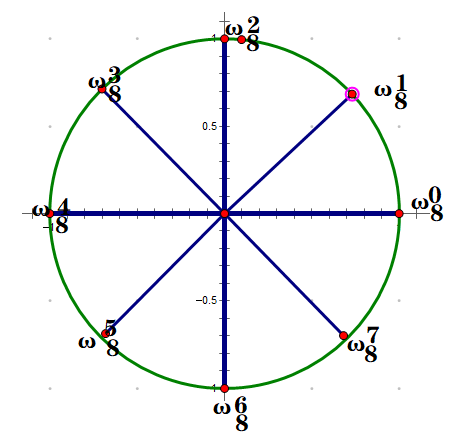
\includegraphics[width=0.5\linewidth]{pic/unitroot.png}
        \caption{$n=8$时的单位复根}
    \end{figure}
\end{frame}

\begin{frame}{快速傅里叶变换}
    现在,傅里叶让$N$是$2$的幂次,他想快速求出
    \begin{equation*}
        f(\omega_N^0),f(\omega_N^1),...,f(\omega_N^{N-1})
    \end{equation*}

    \pause
    首先填充数组,对于下标$k>n$,我们让$a_k=0$,现在来把$f(x)$做一点小小的拆分:
    \begin{align*}
        f(x)&=a_0 + a_1x+ a_2x^2 + \cdots + a_{N-1}x^{N-1}\\
        &= (a_0+a_2x^2+\cdots + a_{N-2}x^{N-2}) + x(a_1+a_3x^2+\cdots + a_{N-1}x^{N-2})
    \end{align*}

    \pause
    如果我们令
    \begin{align*}
        P(x)&= a_0+a_2x+ a_4x^2 + \cdots + a_{N-2}x^{N/2-1}\\
        Q(x)&= a_1+a_3x+ a_5x^2 + \cdots + a_{N-1}x^{N/2-1}
    \end{align*}

    \pause
    那么,$f(x)=P(x^2)+xQ(x^2)$
\end{frame}

\begin{frame}
    对于$0\leq k <\frac{N}{2}$,我们可以算出:
    \begin{equation*}
        f(\omega_N^k)=P(\omega_N^{2k})+\omega_N^{k} Q(\omega_N^{2k})=P(\omega_{N/2}^{k})+\omega_N^{k} Q(\omega_{N/2}^{k})
    \end{equation*}
    
    同理
    \begin{equation*}
        f(\omega_N^{N/2+k})=P(\omega_N^{N+2k})+\omega_N^{N/2+k} Q(\omega_N^{N+2k})=P(\omega_{N/2}^{k})-\omega_N^{k} Q(\omega_{N/2}^{k})
    \end{equation*}

    \pause
    所以说,我们只要计算出
    \begin{align*}
        &P(\omega_{N/2}^0),P(\omega_{N/2}^1),\cdots , P(\omega_{N/2}^{N/2-1})\\
        &Q(\omega_{N/2}^0),Q(\omega_{N/2}^1),\cdots , Q(\omega_{N/2}^{N/2-1})
    \end{align*}

    就可以$O(N)$地算出全部的
    \begin{equation*}
        f(\omega_N^0),f(\omega_N^1),...,f(\omega_N^{N-1})
    \end{equation*}

    \pause
    分治!复杂度?
    \pause
    $T(n)=2T\left(\frac{n}{2}\right)+O(n)=O(n\log n)$
\end{frame}

\begin{frame}[fragile]{FFT(递归版)}
    \begin{lstlisting}[language=c++]
    void FFT(vector<Comp> &a)
    {
        int n=a.size();
        if(n==1) return a;  //多项式只剩1项时,点值等于常数项
        vector<Comp> a1,a2;
        for(int i=0;i<n;i++)  //将f按奇偶项拆分成两个多项式
            if(i&1) a2.pb(a[i]);
            else a1.pb(a[i]);
        FFT(a1); FFT(a2);  //递归处理子问题
        Comp wn=Comp(cos(2*pi/n), sin(2*pi/n)); //单位复根
        Comp w=Comp(1,0);
        for(int i=0;i<n/2;i++)
        {
            Comp x=a1[i],y=a2[i];
            a[i]=x+w*y;
            a[n/2+i]=x-w*y;
            w=w*wn;  //注意:w(n,k+1)=w(n,k)*w(n,1)
        }
    }
    \end{lstlisting}
\end{frame}

\begin{frame}{蝶形变换}
    好心的出题人并不会让你的递归FFT顺利通过,因为递归版FFT的空间复杂度同样达到了$O(n\log n)$,我们需要一个非递归版本的FFT。

    考虑模拟分治过程中的多项式拆分:
    \begin{equation*}
        \begin{array}{cccccccc}
            \{a_0 & a_1 & a_2 & a_3 & a_4 & a_5 & a_6 & a_7\} \\
            \{a_0 & a_2 & a_4 & a_6\} & \{a_1 & a_3 & a_5 & a_7\} \\
            \{a_0 & a_4\} & \{a_2 & a_6\} & \{a_1 & a_5\} & \{a_3 & a_7\}\\
            \{a_0\} & \{a_4\} & \{a_2\} & \{a_6\} & \{a_1\} & \{a_5\} & \{a_3\} & \{a_7\}
        \end{array}
    \end{equation*}

    \pause
    可以看到,最终$a_i$与$a_{R[i]}$发生了位置互换,并且我们可以证明$R[i]$就是$i$的二进制反转!例如:
    \begin{equation*}
        i=6=(110)_2,\quad R[i]=(011)_2=3
    \end{equation*}
\end{frame}

\begin{frame}{蝶形变换}
    直接对每个$i$算出$R[i]$是可行的。当然我们有更快的方法计算$R[0],R[1],...,R[N-1]$

    \pause
    考虑从小到达枚举$i$,这样我们在计算$R[i]$的时候,$R[i/2]$就已经计算好了,我们记
    \begin{equation*}
        i=(B_1B_2B_3...B_l)_2,\quad i/2=(0B_1B_2...B_{l-1})_2
    \end{equation*}

    于是
    \begin{equation*}
        R[i/2]=(B_{l-1}...B_2B_10)_2
    \end{equation*}

    \pause
    除掉末位:
    \begin{equation*}
        R[i/2]/2=(0B_{l-1}...B_2B_1)_2
    \end{equation*}

    \pause
    如果再把首位改成$B_l$,就得到了$R[i]$。只需让上式对$B_l<<(l-1)$按位或即可,因此
    \begin{equation*}
        R[i]=(R[i/2]/2)|((i\&1)<<(l-1))
    \end{equation*}

    这样就可以$O(n)$求出全部$R[0],...,R[N-1]$
\end{frame}

\begin{frame}[fragile]{FFT(非递归版)}
    \begin{lstlisting}[language=c++]
    void FFT(Comp *a)
    {
        for(int i=0;i<n;i++) r[i]=(r[i/2]/2)|((i&1)<<(l-1));
        for(int i=0;i<n;i++) if(i<r[i]) swap(a[i],a[r[i]]);
        for(int i=1;i<n;i*=2)
        {
            Comp wn=Comp(cos(pi/i),sin(pi/i));
            int p=i*2;
            for(int j=0;j<n;j+=p)
            {
                Comp w=Comp(1,0);
                for(int k=0;k<i;k++)
                {
                    Comp x=a[j+k],y=w*a[i+j+k];
                    a[j+k]=x+y;a[i+j+k]=x-y;
                    w=w*wn;
                }
            }
        }
    }
    \end{lstlisting}
\end{frame}

\begin{frame}{FFT的逆变换}
    现在我们已经用$O(n\log n)$的时间求出了
    \begin{align*}
        & f(x_1), f(x_2), ..., f(x_N)\\
        & g(x_1), g(x_2), ..., g(x_N)
    \end{align*}

    接下来我们用$O(n)$的时间计算出
    \begin{align*}
        h(x_1)=f(x_1)g(x_1),\;h(x_2)=f(x_2)g(x_2),...,\;h(x_N)=f(x_N)g(x_N)
    \end{align*}

    最后,我们需要用这些值求出$h$的各项系数。这一步正好和FFT相反,我们称之为IFFT。
\end{frame}

\begin{frame}{FFT的逆变换}
    为简单起见,我们记$\omega=\omega_N$,从形式上,我们有:
    \begin{equation*}
        \begin{bmatrix}
            f(\omega^0)\\
            f(\omega^1)\\
            f(\omega^2)\\
            \vdots\\
            f(\omega^{N-1})
        \end{bmatrix}=
        \begin{bmatrix}
            1 & 1 & 1 & \cdots & 1\\
            1 & \omega & \omega^2 & \cdots & \omega^{N-1}\\
            1 & \omega^2 & \omega^4 & \cdots & \omega^{2N-2}\\
            \vdots & \vdots & \vdots & \ddots & \vdots \\
            1 & \omega^{N-1} & \omega^{2N-2} & \cdots & \omega^{(N-1)^2}
        \end{bmatrix}
        \begin{bmatrix}
            a_0\\
            a_1\\
            a_2\\
            \vdots\\
            a_{N-1}
        \end{bmatrix}
    \end{equation*}

    我们记上面的矩阵为$M$,也就是说$v=\text{fft}(a)=Ma$,那么如果已知左边的向量$v$,要计算$a$,我们有$a=M^{-1}v$
\end{frame}

\begin{frame}{FFT的逆变换}
    \small
    事实上,我们有
    \begin{equation*}
        M=\begin{bmatrix}
            1 & 1 & 1 & \cdots & 1\\
            1 & \omega & \omega^2 & \cdots & \omega^{N-1}\\
            1 & \omega^2 & \omega^4 & \cdots & \omega^{2N-2}\\
            \vdots & \vdots & \vdots & \ddots & \vdots \\
            1 & \omega^{N-1} & \omega^{2N-2} & \cdots & \omega^{(N-1)^2}
        \end{bmatrix}
    \end{equation*}

    \begin{equation*}
        M^{-1}=\frac{1}{N}\begin{bmatrix}
            1 & 1 & 1 & \cdots & 1\\
            1 & \bar\omega & \bar\omega^2 & \cdots & \bar\omega^{N-1}\\
            1 & \bar\omega^2 & \bar\omega^4 & \cdots & \bar\omega^{2N-2}\\
            \vdots & \vdots & \vdots & \ddots & \vdots \\
            1 & \bar\omega^{N-1} & \bar\omega^{2N-2} & \cdots & \bar\omega^{(N-1)^2}
        \end{bmatrix}
    \end{equation*}

    只需要验证$MM^{-1}=I$,也就是说验证$M$的第$i$行与$M^{-1}$的第$j$列向乘,在$i=j$时结果为$1$,在$i\neq j$时结果为$0$

    所以只需把FFT中用到的$\omega$换成$\bar \omega$,最后再把结果乘$\frac{1}{N}$,就得到了IFFT
\end{frame}

\begin{frame}[fragile]{FFT(非递归版)}
    \small
    我们可以把代码改成这样,$v=1$时就是FFT,$v=-1$时就是IFFT

    \begin{lstlisting}[language=c++]
    void FFT(Comp *a, int v)
    {
        for(int i=0;i<n;i++) r[i]=(r[i/2]/2)|((i&1)<<(l-1));
        for(int i=0;i<n;i++) if(i<r[i]) swap(a[i],a[r[i]]);
        for(int i=1;i<n;i*=2)
        {
            Comp wn=Comp(cos(pi/i), v*sin(pi/i)); //这里乘上v就达到了目的
            int p=i*2;
            for(int j=0;j<n;j+=p)
            {
                Comp w=Comp(1,0);
                for(int k=0;k<i;k++)
                {
                    Comp x=a[j+k],y=w*a[i+j+k];
                    a[j+k]=x+y;a[i+j+k]=x-y;
                    w=w*wn;
                }
            }
        }
    }
    \end{lstlisting}
\end{frame}

\begin{frame}[fragile]{多项式乘法}
    借助上面的代码,我们可以很轻松地计算多项式乘法

    \begin{lstlisting}[language=c++]
FFT(a,1);FFT(b,1); //第一步:多点求值(FFT)
for(int i=0;i<=n;i++) a[i]=a[i]*b[i];  //第二步:各点乘积
FFT(a,-1); //第三步:多点插值(IFFT)
for(int i=0;i<=m;i++) printf("%d ",(int)round(a[i].real()/n)); //这里记得要除n
    \end{lstlisting}
\end{frame}

\begin{frame}{例题选讲:高精度乘法}
    \small
    FFT的一个重要应用就是高精度乘法。对于两个数
    \begin{equation*}
        a=a_n...a_3a_2a_1, b=b_m...b_3b_2b_1
    \end{equation*}

    \pause
    如果用模拟的方法,需要两重循环,复杂度为$O(n^2)$。但假如我们写成
    \begin{align*}
        a&= a_1 + a_2\times 10 + a_3\times 10^2 + \cdots  + a_n\times 10^{n-1}\\
        b&= b_1 + b_2\times 10 + b_3\times 10^2 + \cdots  + b_m\times 10^{m-1}
    \end{align*}

    \pause
    我们现在可以使用多项式乘法,令
    \begin{align*}
        f(x)&= a_1 + a_2 x + a_3 x^2 + \cdots  + a_n x^{n-1}\\
        g(x)&= b_1 + b_2 x + b_3 x^2 + \cdots  + b_m x^{m-1}
    \end{align*}

    用FFT算出$h(x)=f(x)g(x)$,得到:
    \begin{equation*}
        h(x)=c_1 + c_2\times x + c_3\times x^2 + \cdots  + c_{n+m-2}\times x^{n+m-2}
    \end{equation*}

    \pause
    有一些$c_k$可能$\geq 10$,因此直接不能直接输出$c_{n+m-2}...c_2c_1$,要再做一次进位,复杂度$O(n+m)$。
\end{frame}

\begin{frame}{例题选讲:高精度连乘}
    \small
    给$n$个数$c_1,c_2,...,c_n$,求$c_1\times c_2\times \cdots \times c_n$

    $n\leq 10^5$,$1\leq c_i\leq 9$

    \pause\vspace{1em}
    能不能用高精度乘法的方法,计算$c_1\times c_2$,然后乘$c_3$,再乘$c_4$,再乘$c_5$……?

    \pause\vspace{.5em}
    不能!复杂度$O(n^2)$

    \pause\vspace{.5em}
    【题解】令$M(l,r)=c_l\times c_{l+1}\times \cdots \times c_r$,显然我们要求的就是$M(1,n)$,考虑分治。

    \pause
    递归计算$M(1,n/2)$,$M(n/2+1,n)$,然后
    \begin{equation*}
        M(1,n)=M(1,n/2) \times M(n/2+1,n)
    \end{equation*}

    这一步用FFT优化,复杂度是$O(n\log n)$,分治总复杂度为$T(n)=2T(n/2)+O(n\log n)=O(n\log^2 n)$
\end{frame}

\begin{frame}{例题选讲:带通配符的字符串匹配}
    请移步洛谷P4173

    第一篇获赞100+的题解是我五年前写的。
\end{frame}

\section{参考文献}

\begin{frame}[allowframebreaks]
    \bibliography{ref}
    \bibliographystyle{ieeetr}
    \nocite{*} % used here because no citation happens in slides
    % if there are too many try use:
    % \tiny\bibliographystyle{alpha}
\end{frame}


\begin{frame}
    \begin{center}
        {\Huge\calligra Thank You}
    \end{center}
\end{frame}

\end{document}